\chapter{Introduction}
There is an increasing awareness of the potential benefits of intelligent energy control. Indeed, intelligent control
of the balance between the distributed energy resources and the demand requirements has many advantages. It leads to efficient planning, more satisfied customers and can even help national electricity markets in saving considerable operating and maintenance costs \cite{NarjesFallah2018}. Having accurate forecasting models is one of the key conditions to realize intelligent energy control. When electricity consumption forecasting is improved, energy suppliers can build a better trust with their customers by sending reliable bills. Furthermore, the electricity supplier can better estimate the energy demand of the whole customer population. The optimization of the energy production planning is possible, which will lead to cheaper electricity production and increased profit margins. More substantiated decisions can be taken with regard to investments and there will be less need of the more flexible, but more expensive electricity installations e.g. diesel engines, to catch the deficiencies in electricity production.\\

\begin{figure}[h!]
	\centering
	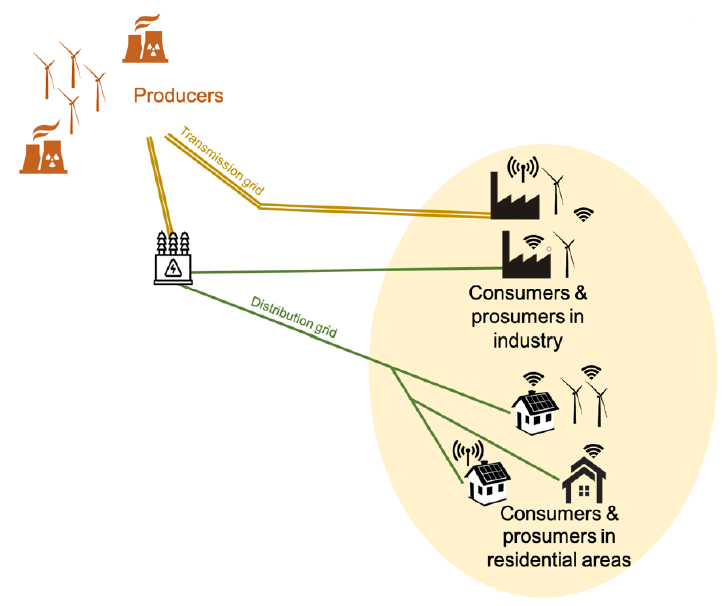
\includegraphics[width=0.8\textwidth]{SmartGrid.png}
	\caption{Electricity grid (Source: KU Leuven thesis proposal).}
	\label{fig:power_image}
\end{figure}

With the invention of the smart meter in 1974 by \textbf{Paraskevakos}, it became possible to measure the electricity consumption with a higher accuracy and communicate this with the electricity consumer and producer. Electricity consumption is nearly recorded real time and a smart meter allows for two-way communication between the smart meter and the supplier. As explained in \cite{Depuru2011}: ``By introducing smart meters as a new
component of their smart grid system, an avalanche of immensely useful energy usage information
became available to the energy markets.'' From the availability of more detailed datasets comes the explosion of research in the area of electrical forecasting techniques and the applicability of more complex models. To tackle the electrical consumption forecasting problem neural networks are applied. These models allow for learning non-linear relations between the inputs and outputs.\\

\begin{table}[h!]
	\centering
	\begin{tabular}{@{}lp{3cm}p{3cm}p{4.5cm}@{}} \toprule
		\textbf{Acronym}	& \textbf{Prediction type} & \textbf{Time span} & \textbf{Application}\\\midrule
		VSTLF	& Very short Term Load Forecasting	& One minute to an hour	& Operational and maintenance
		scheduling and Demand side management
		(decision making for load
		control and voltage reduction)\\\hline		
		STLF	&	Short Term Load Forecasting 	& 	Daily or weekly		& Distribution and transmission
		planning and Demand side management
		(decision making for load
		control and voltage reduction)\\\hline	
		MTLF	&	Medium Term Load Forecasting	& A month to a few years	& Finance or power supply planning\\\hline
		LTLF	&	Long Term Load Forecasting	&	A year to a few decades	&	Finance or power supply planning\\\bottomrule
	\end{tabular}
	\caption{Prediction types \cite{NarjesFallah2018}.}
	\label{tab:prediciontypes}
\end{table}

Depending on the forecasting horizon, different applications are considered, as is summarized in Table \ref{tab:prediciontypes} \cite{NarjesFallah2018}. The forecast horizon is chosen in consultation with the uncertainty that is contained in the signal. If the signal doesn't show clear patterns, forecasting will be more difficult which means that the forecasting horizon should be shorter. In this thesis the forecasting horizon falls in the category of ``VSTLF'' and ``STLF'' because the consumption is predicted with time steps of 30 minutes and 24 hours ahead. The practical application of the developed models in this thesis have as goal to monitor the demand side of the low voltage distribution grid. Figure \ref{fig:power_image} shows in green where the distribution grid is located in the whole electricity grid. The low voltage distribution grid is also called the secondary network and is the part of the distribution grid that carries electric energy from distribution transformers to the electrical appliances located in a house. Typical inputs that are used in literature for electrical load forecasting are past values of the load, weather information, calendar information and error-correction terms \cite{loadforecastingmoor}. Often used inputs for electrical load forecasting are summarized here.

\begin{itemize}
	\item Historical data e.g. \cite{Kong2019}
	\item Weather information
	\begin{itemize}
		\item Temperature e.g. \cite{Kong2019}
		\item Cloudiness e.g. \cite{Contaxi2006}
		\item Humidity e.g. \cite{Contaxi2006}
		\item Wind e.g. \cite{Charytoniuk1997}
	\end{itemize}
	\item Day of the week e.g. \cite{Kong2019}
	\item Time of the day e.g. \cite{Kong2019}
	\item Holiday e.g. \cite{Kong2019}
	\item Anthropological data : Social aspects of the community, general behaviour of house
	occupants e.g. \cite{Javed2012}
	\item Structural data : physical properties of the house e.g. \cite{Javed2012}
\end{itemize}

\section{Importance of topic}
This research on short term load forecasting is done in the context of an increased adoption of solar panels and electric vehicles by the general public. Every year 40000 new solar panel installations take place in Flanders \cite{Lemmens2019}. Fluvius, which is one of the Belgian distribution grid operators, has carried out, together with Deloitte in 2019, an unique stress test on the low voltage distribution grid to analyse how the current grid would react on an increased amount of charging points for electrical vehicles and solar panels. It was found that on the short term, which means up to 2025, the grid will be able to cope with the estimated increase of the burden on the low voltage grid. However, now is the time of anticipation and to strengthen the weak spots in the network. To carry out the maintenance work, detailed forecasting of the load signals of only a small amount of households is needed. Detailed forecasts of individual households is now possible thanks to the use of smart meters. If detailed predictions can be achieved for individual households, expenses are saved because customized updates of the network can be done. With forecasts on the household level, a plan can be made where only certain parts of the grid have to be replaced. Replacing everything is avoided. Individual household predictions can be used as part of a congestion prediction, which means predicting when the low voltage grid can't handle the demand anymore. In that case, a precise prediction of the size and time of peaks is crucial. If an accurate congestion prediction can be done, the reliability of the network increases and the risk for blackouts and brownouts is decreased.\\

\section{Problem formulation and link with previous studies}
As discussed in \cite{Shi2018}, the complexity of the household forecasting lies in the significant uncertainty and volatility of the load signal. Uncertainty comprises the aperiodic part influenced by external factors e.g. customer behaviour and weather.In order to attain accurate forecasting results, it is found in literature that aggregated load signals are considered \cite{loadforecastingmoor}. Aggregation cancels out the individual uncertainty, and the signal will show a higher periodicity, which is easier to model. However, this doesn't help for individual household forecasting. Papers about load forecasting of an individual household often use a lot of information about the household situation and submeters to measure the consumption of different appliances or parts of the house \cite{Kim2019}. This will in practise not be scalable due to privacy concerns, among other things. This thesis investigates state of the art time series short term forecasting techniques based on LSTM neural networks that have as goal to directly learn the uncertainties on the load signals, given only limited information.\\


The data used in this thesis was made available for the \href{https://ieee-dataport.org/competitions/ieee-cis-technical-challenge-energy-prediction-smart-meter-data}{IEEE-CIS technical challenge on energy prediction from smart data} and is very similar to smart meter data from the Belgian Energy supplier Fluvius.
This dataset consists out of 3248 smart meter time series form the UK during the year 2017. 

\section{Thesis objective and structure}
The goal of this thesis is to implement short-term load forecasting for individual households when using only a limited amount of information. Firstly, the following question will be answered : ``How much electricity will a individual household consume in the next 24 hours?'' LSTM neural networks are investigated to predict a load signal of 24 hours ahead with time steps of 30 minutes. The information used to make the predictions consists of past load values, calendar information and the daily average temperature of tomorrow. These inputs can easily be obtained in practice without intruding the privacy of the residents. The three households considered, originate form the IEEE-CIS technical challenge dataset. The results of this research are interesting, because real-life data is used. However, the development of the models is more challenging due to the anomalies and missing values that are present in the data. The second part of the thesis objective is to evaluate the forecasting performance of the different developed models. To be able to develop the models I had to get familiar with: scikit-learn, Jupyter Notebook, Tensorflow, Keras, Pandas, Anaconda and Microsoft Azure. Therefore, completing this thesis was an educational experience that improved my software skills.\\ 

This report is divided in 4 chapters, followed by the conclusion and the appendix. First, an exploratory data analysis conducted on the dataset from the IEEE-CIS technical challenge is presented in Chapter \ref{cha:Data analysis}. The goal is to determine the general characteristics of the data. 261 load series, with a full year of measurements are assessed. In section \ref{s:Preprocessing} the missing values, zero days, normalization and shifts in the rolling mean loads are discussed. In Section \ref{s:Data Analysis} the selected load series with a full year of smart meter measurements are aggregated to identify general characteristics of the data. In this section seasonality, comparison between weekdays and weekends, impact of an holiday on the load signal, influence of the temperature and the identification of the influence of properties of the household e.g. dwelling type is analysed. The additional household properties considered in the last analysis were available through a voluntary questionnaire. \\
In Chapter \ref{cha:State of the art short-term residential load forecasting techniques} the literature study is explained. First, an introduction is given about neural networks. The challenges and solutions are discussed in Section \ref{s:Problems}. The advanced LSTM and GRU neural networks are detailed in Section \ref{s:LSTM} and \ref{s:GRU} respectively. These networks are specialized in the handling of time series. The introduction to neural networks ends with an explanation concerning the performance of different parameter settings and different LSTM architectures in Section \ref{s:Performance results between different models}. The second part of the literature study covers the use of LSTM models for short-term residential electrical load forecasting in Section \ref{s:Short-Term residential electrical load forecasting}.\\
In Chapter \ref{cha:Forecasting the daily electricity consumption}, three households are selected from the IEEE-CIS technical challenge dataset. The corresponding load signals are used for individual household forecasting. In section \ref{s:Preprocessing_cha4}, the raw data is introduced and the preprocessing is detailed. Section \ref{s:Error metrics} discusses the error metrics used to evaluate the prediction performance of the models. Section \ref{s:Microsoft Azure cloud} clarifies how Microsoft Azure is used for cloud computing. Section \ref{s:Baseline models} describes the development of baseline models that serve as a benchmark for the advanced Deep LSTM models which are explained in Section \ref{s:Deep LSTM neural networks}. In Section \ref{s:Implementation deep LSTM neural network} the developed Deep LSTM models are discussed and a parameter search is conducted. Chapter \ref{cha:Model evaluation} shows the results of the LSTM models on the test set with respect to the baseline models. The conclusion of this work is presented in Chapter \ref{cha:conclusion}.





%%% Local Variables: 
%%% mode: latex
%%% TeX-master: "thesis"
%%% End: 
